% LTeX: language=de-DE
\chapter{Elektronik}
	Die verwendeten ESC sind in der Lage die rückwirkende elektromotirische Kraft (rEMK\nomenclature[A]{rEMK}{Rückwirkende elektromotorische Kraft}) --~eine während des Betriebes in den Wicklungen des Motors erzeugte und seiner Drehrichtung entgegenwirkenden Spannung -- zu Messen und zur Positionsbestimmung des Rotors zu nutzen.
	Gegenüber eines trapezoidalen Phasenstromes können die Motorwicklungen so sinusoidal bestromt werden, was wiederum geringere elektrische Verluste und ein gleichmäßigeres Drehmomentprofil während eines Umlaufes und damit einen sanfteren und geräuschärmeren Motorlauf verspricht.
	Prinzipbedingt steigt die Amplitude der rEMK mit der Drehzahl des Motors.
	Konsequenterweise wird so die Messung und damit die Positionsbestimmung im niedrigen Drehzahlbereich erschwert während sie im Stillstand unmöglich wird.
	Um ein exaktes Feedback der Rotorposition an die Steuerelektronik unabhängig der rEMK zu ermöglichen, verfügen die ausgewählten Motoren über integrierte Hall-Effekt-Sensoren.
	Im höheren Drehzahlbereich verschwinden ihre Vorteile zwar zunehmend, liefern jedoch die Möglichkeit eines äußerst sanften Anlaufes aus dem Stillstand heraus.\par\medskip
	%
	\begin{wrapfigure}{r}{.5\textwidth}
		\centering
		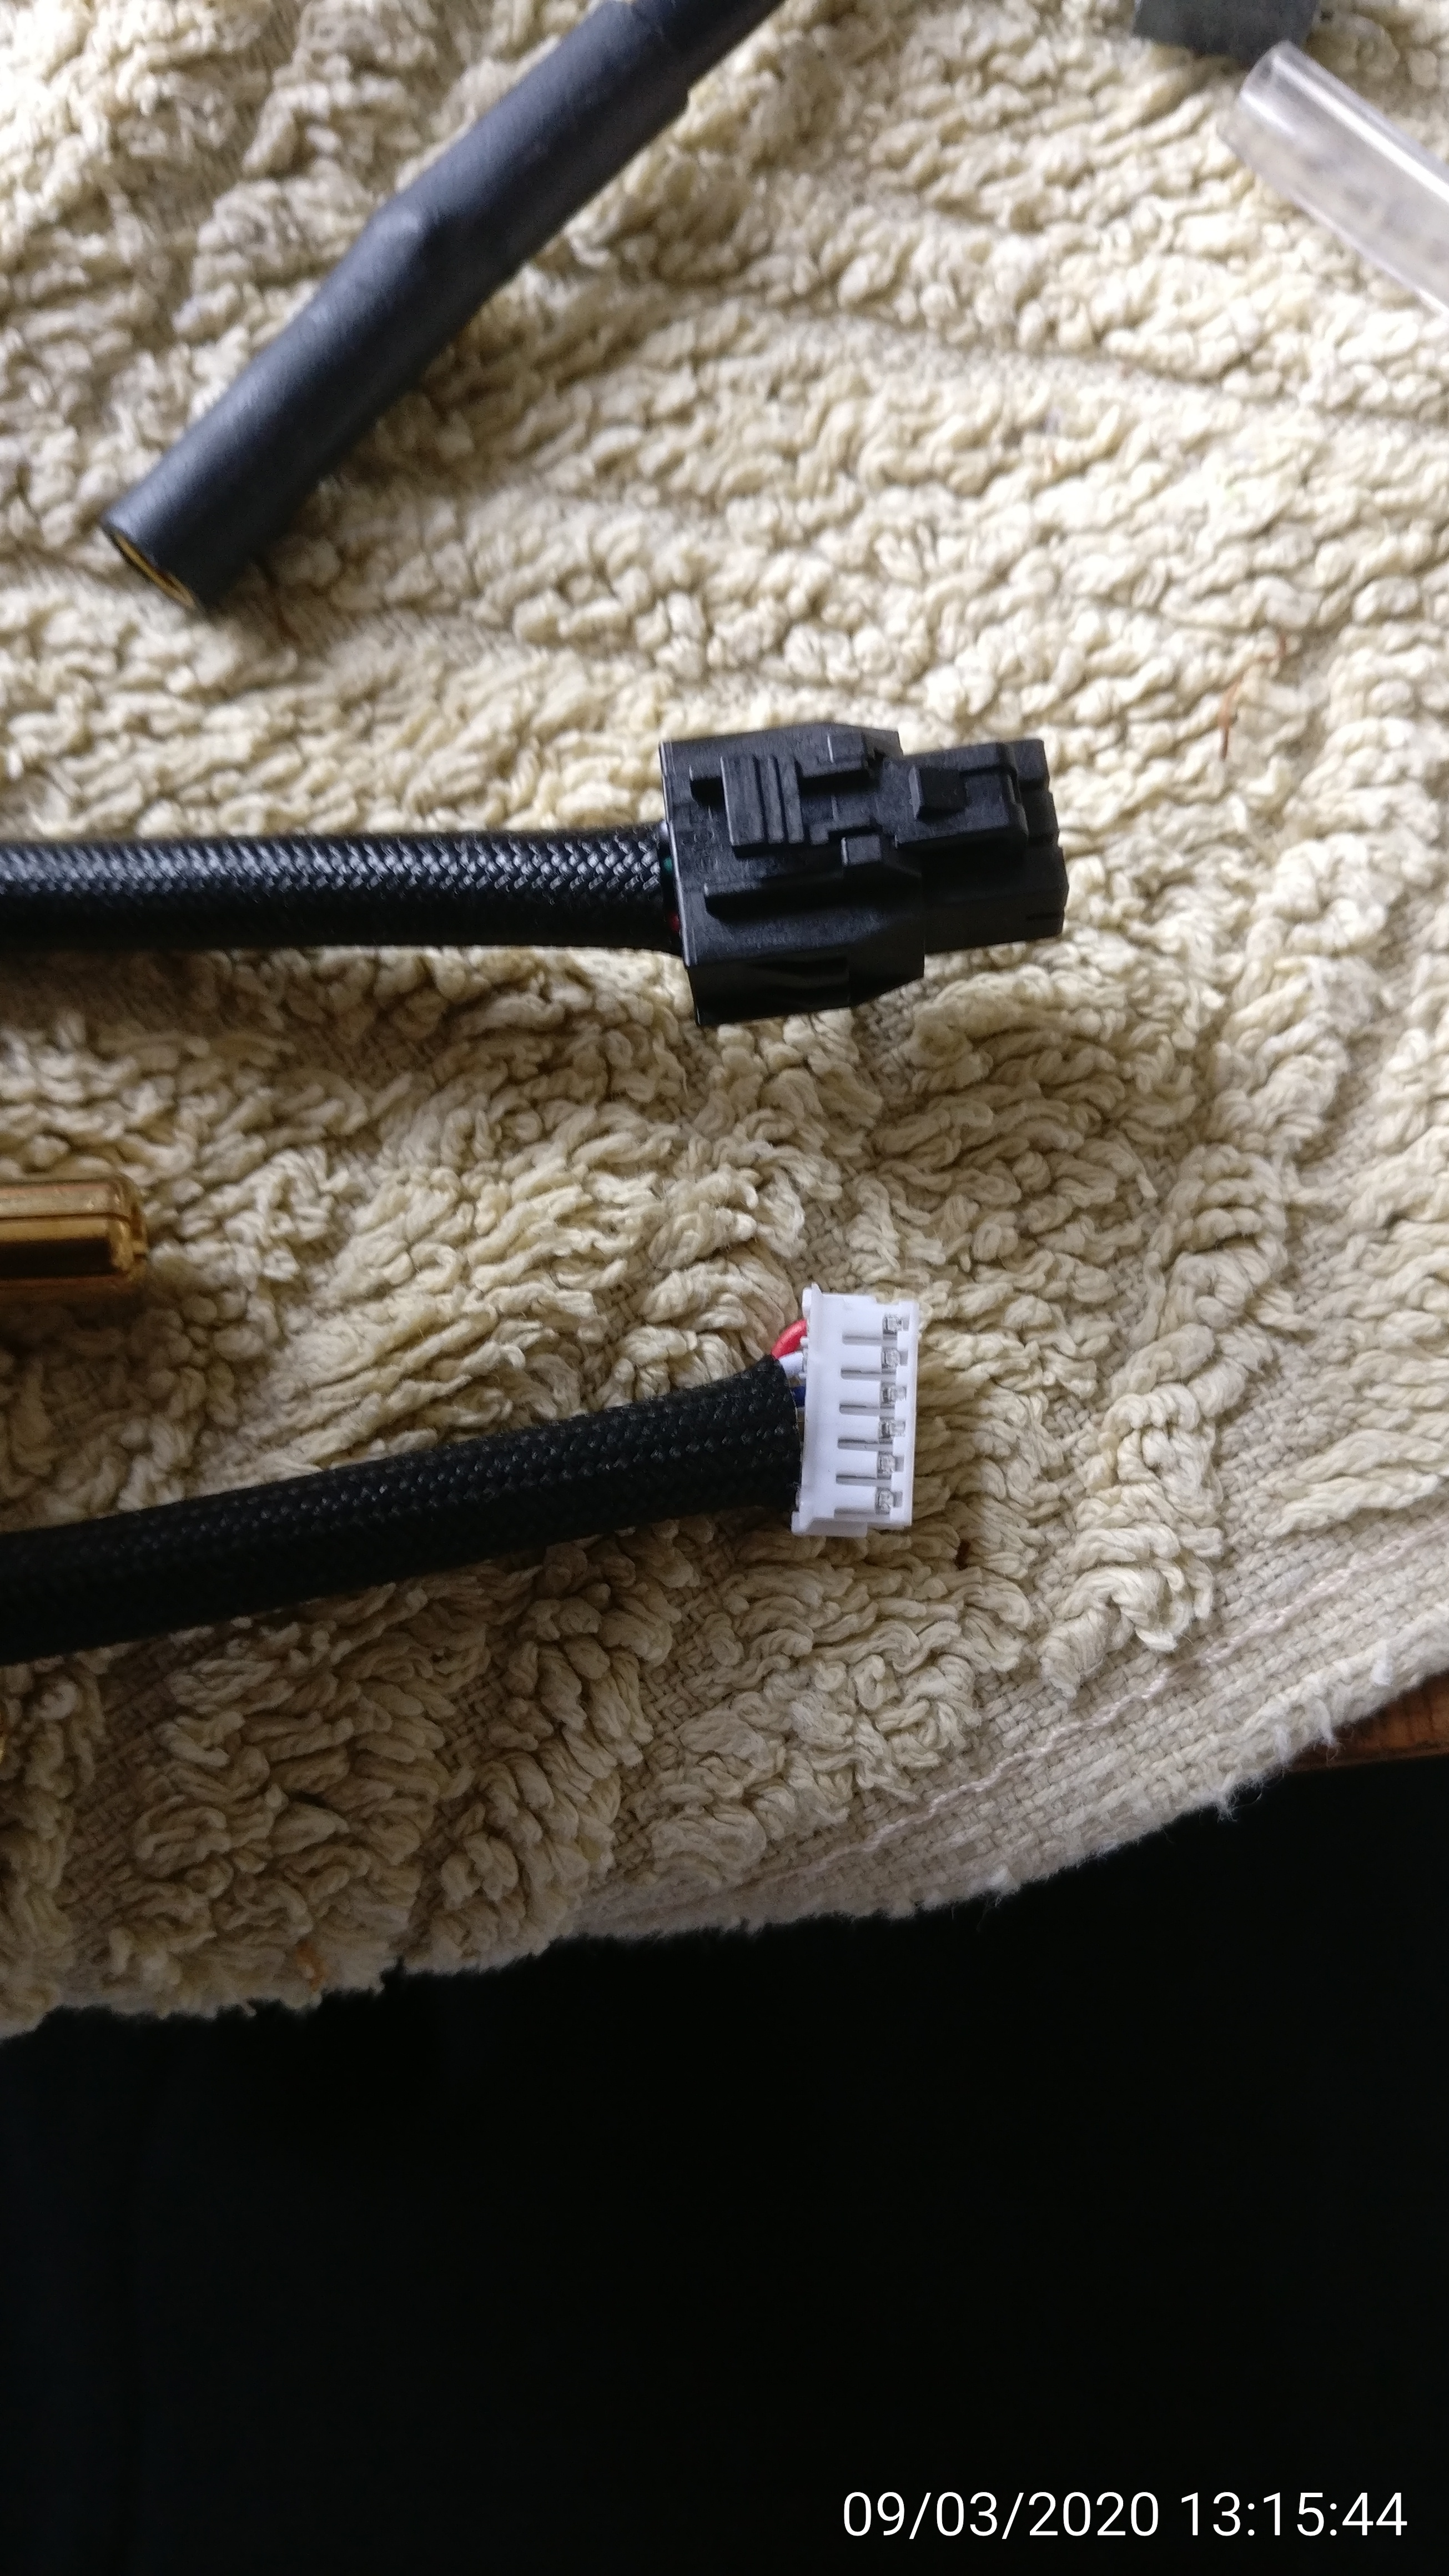
\includegraphics[angle=90, width=.4\textwidth]{Footage/Pictures/Hall sensor connector.jpg}
		\caption[Hall-Sensoren Konnektoren]{Links ein 3x2-Pin Molex Micro-Fit 3.0 Konnektor, rechts ein 6-Pin JST-PH zur Verbindung mit dem ESC.}
		\label{fig:hall sensor connectors}
	\end{wrapfigure}
	Die ab Werk unterminierten Sensorenleitungen wurden im Sinne einer Staub- und Spritzwassergeschützen Durchführung in das GFK-Gehäuse über eine Kabelbrücke mit den ESC verbunden.
	Die Kabelbrücke wurde aus 30AWG\nomenclature[A]{AWG}{American Wire Gauge}\footnote{Entspricht etwa \qty{0,25}{\milli\metre\squared}.} flexibler Silikonleitung mit einem 6-Pin JST-PH Konnektor ESC-seitig und einem 3x2 Molex Micro-Fit 3.0 Konnektor motorseitig gefertigt (vgl. \cref{fig:hall sensor connectors}).
	Für den motorseitigen Anschluss wurde eine entsprechende Öffnung in das Gehäuse geschnitten und der Konnektor mit Epoxidharz dauerhaft und dicht verbunden.
	Die Anordnung der Sensoren spielt an dieser Stelle eine untergeordnete Rolle, da sie vor Inbetriebnahme softwareseitig konfiguriert werden können.
	Es wird lediglich darauf geachtet, dass die Anordnung beider Motoren identisch bleibt.
	Zur Durchführung der Phasenleitungen werden je Motor drei Löcher in das Gehäuse gebohrt und mit Gummiösen versehen.\par\medskip
	%
	Die hardwareseitige Leistungsendstufe ist als Doppel-H-Brücke implementiert und in \cref{fig:power mosfets} gezeigt.
	Um den Rotor um \qty{360}{\degree} dividiert durch die Anzahl der Polpaare \(n_\text{p}\)\nomenclature[L]{\(n_\text{p}\)}{Anzahl der Polpaare\nomunit{1}} zu drehen, muss ein voller Kommutationszyklus durchgeführt werden, was im Folgenden einer elektrischen Umdrehung entsprechen soll.
	Die Anzahl elektrischer Umdrehungen je Minute bei gegebener mechanischer Drehzahl des Rotors sei somit gegeben durch:
	\begin{align}
		\omega_\text{e} = \omega n_\text{p}
		\label{eq:ERPM and RPM}
	\end{align}
	\nomenclature[G]{\(\omega_\text{e}\)}{Elektrische Drehzahl\nomunit{\per\minute}}
	\nomenclature[G]{\(\omega\)}{Mechanische Drehzahl\nomunit{\per\minute}}
	%
	Die Maximalgeschwindigkeit skaliert somit direkt proportional mit \(\omega_\text{e}\) nach
	\begin{align}
		v_\text{max} = \omega_\text{e} \frac{2\pi r}{n_\text{p} \zeta}
		\label{eq:max speed by ERPM}
	\end{align}
	Die Konfigurationssoftware der ESC lässt zu, dass ein oberer Grenzwert für \(\omega_\text{e}\) und damit unmittelbar für die Maximalgeschwindigkeit definiert werden kann.

	% Die technische Dokumentation der ESC empfiehlt, \(ERPM\) unterhalb eines Wertes von \num{60000} zu halten.

	% Bei gegebener Batteriespannung und den verwendeten Motoren mit sieben Polpaaren liefert \cref{eq:max rpm} multipliziert mit dem zweifachen der Polpaarzahl ein theoretisches Maximum der ERPM von \num{95760} und liegt damit deutlich über dem empfohlenen oberen Grenzwert.
	% Die ESC verfügen über die Möglichkeit, hier softwareseitig Maximal- und Minimalwerte zu hinterlegen.
	% Mit zusätzlichem Sicherheitsabstand von \qty{10}{\percent} wird ein oberer Grenzwert von \num{54000} festgelegt was einer reduzierten Maximalgeschwindigkeit von etwa \qty{24}{\kilo\metre\per\hour} entspricht.